% ----------------------------------------------------------------------

\chapter{\textbf{Referencial Teórico}} % Este comando é utilizado para criar capítulos
\sloppy % Corrige estouro de linhas

\section{TECNOLOGIA NA EDUCAÇÃO }

O termo ''tecnologia'' diz respeito a muitas outras coisas além das máquinas. O conceito tecnologia engloba a criatividade engenhosa do cérebro humano desde os primórdios da Humanidade. Sua aplicação perpassa pela utilização de diversos recursos naturais, com objetivo de criar ferramentas instrumentais e simbólicas, para transpor barreiras impostas pela natureza até aos testes e aplicação de novas teorias e princípios científicos \cite{kenski2007educaccao}.

A sociedade contemporânea está inserida no momento de constante advento tecnocientífico, e de forma direta e indireta, isto reflete nas práticas pedagógicas escolares. Conforme \citeonline{martins2010gestao}, o educador deve estar sempre atualizado, pois a transformação nos processos tecnológicos e meios de comunicação são permanentes. A presença das TIC (tecnologias de informação e comunicação) na educação é um tema dinâmico e catalisador de transformações no processo ensino-aprendizagem. Estudos demonstram que a condição para o uso com êxito das TIC nas escolas reside, antes de tudo, em saber com utilizá-las e aplicá-las nas atividades curriculares \cite{noeth2004evaluating}. Nesse sentido, a qualificação profissional para o uso das TIC é primordial \cite{david2008padroes}.

De acordo com \citeonline{kenski2007educaccao}, a abordagem didática com integração das TIC no processo ensino-aprendizagem pode alavancar a aprendizagem e o desenvolvimento dos educandos via inserção digital. O grande desafio para escola e educadores, consiste em saber aplicar as TIC como potencializador no sistema educacional, especialmente em seus componentes pedagógicos e processos de ensino-aprendizagem \cite{libaneoorganizacao}.

\section{SISTEMAS DISTRIBUÍDOS}

Na computação moderna vários sistemas computacionais interagem entre si de forma interdependente, sendo a internet o exemplo mais perceptível a ser citado. São várias redes interconectadas e aplicações que fazem uso de tais estruturas para se comunicarem, abrangendo os mais variados domínios. Todas essas estruturas empregam conceitos da tecnologia sistemas distribuídos \cite{puder2011distributed}.\\
\citeonline{tanenbaum2007distributed} descrevem um sistema distribuído como sendo um conjunto de computadores autônomos não obrigatoriamente equivalentes, interligados entre si e compreendidos pelo usuário como um único sistema conexo. Sua compreensão destaca a interdependência e a colaboração entre os computadores como sendo um elemento de suma importância para a existência da arquitetura. A definição proposta por \citeonline[p. 2]{coulouris2005distributed} torna ainda mais precisa através da seguinte definição sobre sistemas distribuídos:

\begin{citacao}
	Definimos um sistema distribuído como aquele no qual os componentes de hardware ou software, localizados em computadores interligados em rede, comunicam-se e coordenam suas ações apenas enviando mensagens entre si.
\end{citacao}

\citeonline{puder2011distributed} destacam vários benefícios dos sistemas distribuídos em comparação com sistemas centralizados, tais como redundância, economia, escalabilidade e tolerância a falhas.

\section{WEB SERVICES}

Considerando as várias utilidades dos sistemas distribuídos, \citeonline{fielding2000} definiu em sua tese de doutorado o REpresentational State Transfer (REST),  um estilo arquitetônico para sistemas hipermídia distribuídos. Tal arquitetura foi desenvolvida com base na disponibilização de recursos, mapeados de forma exclusiva através de URIs (Uniform Resource Identifiers), que são acessadas através de URLs (Uniform Resource Location), funcionando sobre o protocolo HTTP \cite{richardson2008restful}. Em seu trabalho, Fielding destaca seis atribuições básicas que caracterizam o padrão REST, são estas:

\begin{enumerate}
	\item {A aplicação deve utilizar a arquitetura cliente-servidor;}
	\item {Todas as requisições devem ser independentes e isoladas entre si, não havendo nenhum estado de sessão guardado no servidor (Stateless);}
	\item {Requisições já executadas previamente podem ser mantidas em memória para reutilização futura por chamadas equivalentes (Cache);}
	\item {Deve existir uma padronização na manipulação, no mapeamento dos componentes disponibilizados e no formato de troca de dados (Interface Uniforme);}
	\item {O sistema deve ser projetado em camadas, de modo que a interação entre componentes de diferentes camadas seja limitada ao essencial;}
	\item {Código sob demanda, permitindo que applets ou scripts sejam baixados para execução no lado cliente (podendo ser opcional a implementação deste quesito);}
\end{enumerate}

O padrão definido por Fielding se mostra uma alternativa altamente performática em comparação com webservices tradicionais tais como SOAP, principalmente pelo tamanho de mensagens e tempos de resposta menores, tal como afirmam \citeonline{hamad2010} e \citeonline{dudhe2014performance}. A comunidade web e grandes empresas tais como Google e Amazon têm se utilizado dessa tecnologia para construir seus serviços, dado sua simplicidade e escalabilidade \cite{wagh2014hybrid}. REST tem sido amplamente utilizado em conjunto com o JavaScript Object Notation (JSON), uma estrutura de dados simples e leve, em substituição ao formato XML como padrão representativo de troca de dados, sendo suportado pela maioria dos Web Browsers atuais \cite{knutsen2018}.

\begin{figure}[h]
	\caption{Arquitetura de um Web Service RESTful.}
	\caption*{Fonte: \citeonline{thu2015}.}
	\centering % para centralizarmos a figura
	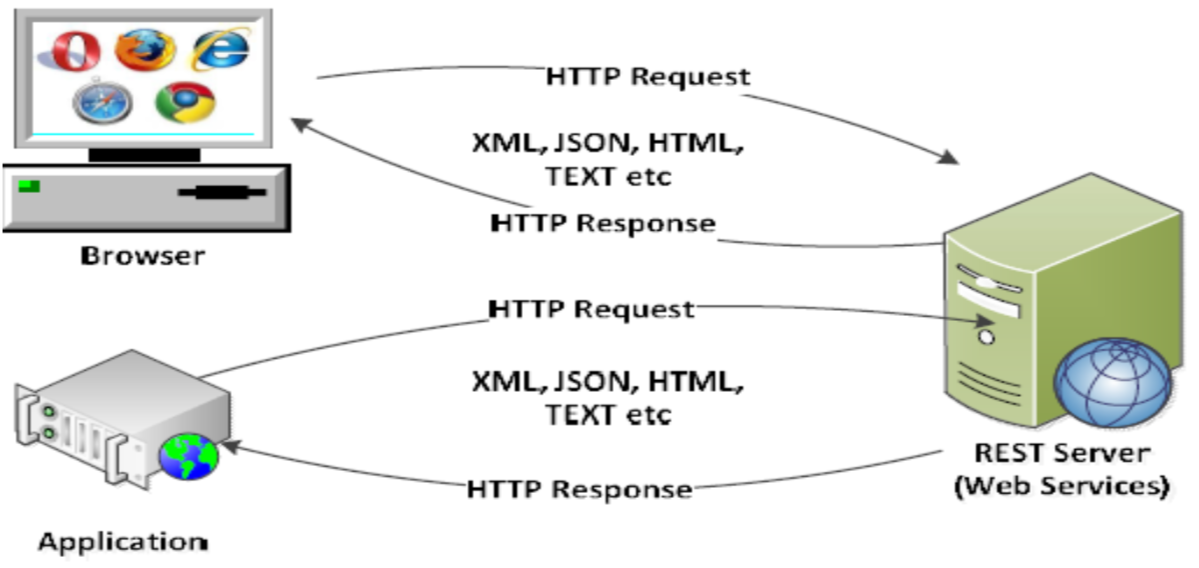
\includegraphics[width=12cm]{resources/webservices.png} % leia abaixo
	\label{figura:webservices}	
\end{figure}

\pagebreak
A figura \ref{figura:webservices} ilustra uma representação básica de um webservice implementado utilizando a arquitetura Rest (RESTful), onde essencialmente são realizadas requisições (HTTP Request) a partir de um determinado cliente (aplicação ou web browser) para um servidor (REST Server), que responde à solicitação com uma resposta (HTTP Response), contendo em seu corpo uma informação padronizada por algum formato representativo de troca de dados (XML, JSON, HTML, TEXT).

\begin{table}[h]
	\captionsetup{justification=centering}
	\centering
	\caption{Métodos HTTP e suas funções correspondentes.}
	\caption*{Fonte: \citeonline{hamad2010}.}
	\label{tabela:metodoshttp}
	\begin{tabular}{r|lr}
		Método HTTP &  Ação\\
		\hline
		GET & Lê um recurso  \\
		POST & Cria um recurso  \\
		PUT & Altera um recurso \\
		DELETE & Deleta um recurso 
	\end{tabular}
\end{table}

Aplicações RESTful utilizam-se dos chamados métodos HTTP para manipulação de dados. A tabela \ref{tabela:metodoshttp} lista os principais métodos e suas respectivas ações, sendo elas leitura, criação, alteração e deleção de dados, respectivamente \cite{pautasso2008restful}.

\section{JSON WEB TOKEN (JWT)}

Quanto à segurança de acesso, web services RESTful podem utilizar mecanismos para garantir que somente usuários autorizados tenham acesso aos recursos. Neste sentido, o padrão JWT (JSON Web Token) \cite{jwt} se mostra uma alternativa concreta para a transmissão de informações confidenciais de autenticação em sistemas stateless \cite{jones2015json}. \citeonline{peyrott2016jwt} descreve tal padrão como um meio simples, compacto e seguro de realizar solicitações, sendo utilizado por uma grande parcela de aplicativos.

\begin{figure}[h]
	\caption{Estrutura básica de um token JWT.}
	\caption*{Fonte: \citeonline{rahmatulloh2018}.}
	\label{figura:jwt}
	\begin{center}
		\textcolor{red}{xxxxxx}.\textcolor{green}{yyyyyyy}.\textcolor{blue}{zzzzzzzz}\\
		\textcolor{red}{header}.\textcolor{green}{payload}.\textcolor{blue}{signature}\\
	\end{center}
\end{figure}

A figura \ref{figura:jwt} ilustra a estrutura básica do JWT, constituída basicamente por uma string de caracteres criptografada denominada Token, dividida em três seções: header, payload e signature.

\section{REDES NEURAIS}

\citeonline{haykin2009neural} descreve o conceito de Redes Neurais utilizando-se do exemplo dos sistemas biológicos naturais, que possuem alta capacidade de aprendizado e conseguem assimilar informações complexas no ambiente ao redor em um curto espaço de tempo. Isto se dá pelo fato de que um computador processa informações de forma diferente de um cérebro humano, por exemplo. Neste escopo, uma rede neural objetiva o mapeamento de tais informações de forma a torná-las acessíveis para utilização.

Para \citeonline{hagan1996neural}, apesar de as as Redes Neurais não apresentarem uma solução para todos os problemas matemáticos e de engenharia, elas tem se mostrado um recurso poderoso em casos apropriados para sua aplicação. Muitos dos seus avanços atuais se devem ao avanço do poder de processamento dos computadores, o que possibilita a realização de testes cada vez mais complexos.

